\section{Normal Sampling}
\subsection{Task A}
To prove that Y is uniformly distributed in [0,1], we need to prove that for an arbitrary interval [a,b] in [0, 1], Y lies in [a, b] with probability $b-a$.\\
The probability that $a \le Y \le b$ is the probability that the randomly chosen X is such that $a \le F_X(x) \le b$. The cumulative probability of x being in the interval $[a_0, b_0]$ such that $F_X(a_0) = a$ and $F_X(b_0) = b$ is $b-a$, since the cumulative probability that $x \le b_0$ is b, and the cumulative probability of $x\le a_0$ is a, hence probability that $a_0 \le x \le b_0$ is $b-a$. Our condition that $F_X()$ is invertible guarantees that the $\le$ can be replaced with $<$, since it cannot be that $\lim_{x\to a_0^-} \ne \lim_{x\to a_0^+}$, otherwise between $a_0^-$ and $a_0^+$, all elements would be mapped to by $a_0$.

\subsection{Task B}
Given a sample y, let us return $F_X^{-1}(y)$. To prove that this has the same CDF as X, we need to prove that if $F_X(a_0)=a$ and $F_X(b_0)=b$, the probability of getting $a_0 \le F_X^{-1}(y) \le b_0$ is $b-a$.\\
But this is fairly straightforward, since $a_0 \le F_X^{-1}(y) \le b_0 \iff a \le y \le b$, and the probability of getting $a \le y \le b$ is $b-a$.\\
Thus, this is the required function.

\subsection{Task C}
Code provided in 2c.ipynb.
\begin{figure}[H]
    \centering
    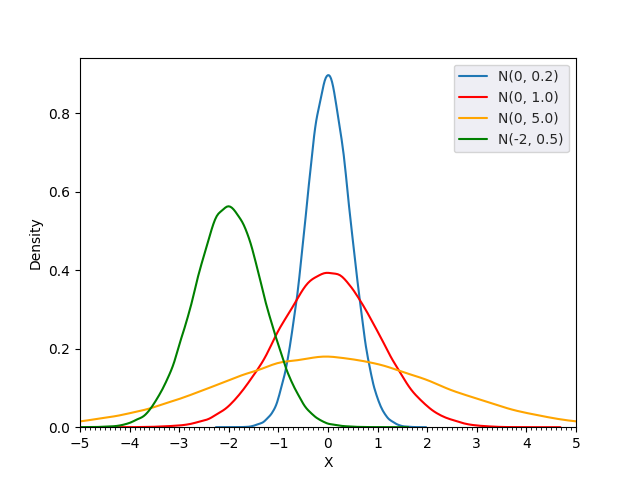
\includegraphics[width=0.6\textwidth]{../images/2c.png}
    \caption{Histogram of the samples generated}
    \label{fig:2c}
\end{figure}

\subsection{Task D}
Code provided in 2d.ipynb.
\begin{figure}[H]
    \centering
    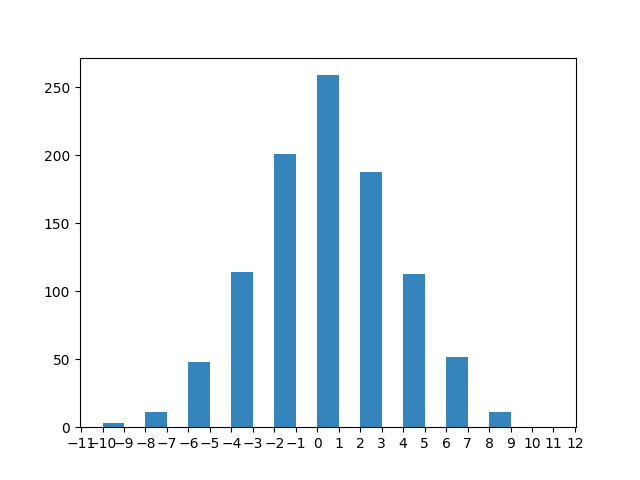
\includegraphics[width=0.6\textwidth]{../images/2d1.png}
\end{figure}
    \begin{figure}[H]
        \centering
        \caption{h=10}
    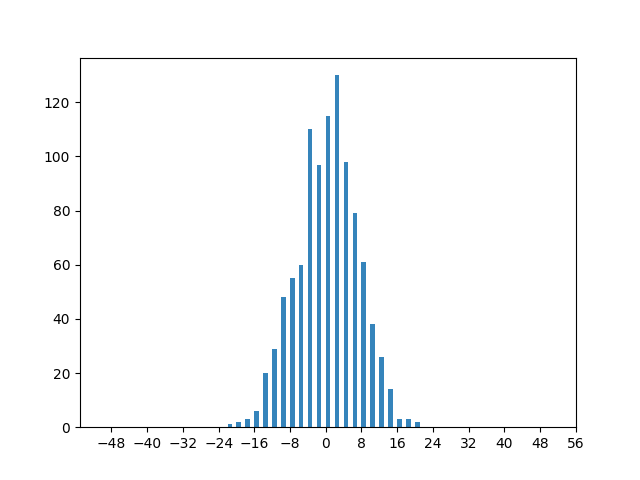
\includegraphics[width=0.6\textwidth]{../images/2d2.png}
    \caption{h=50}
\end{figure}
    \begin{figure}[H]
        \centering
        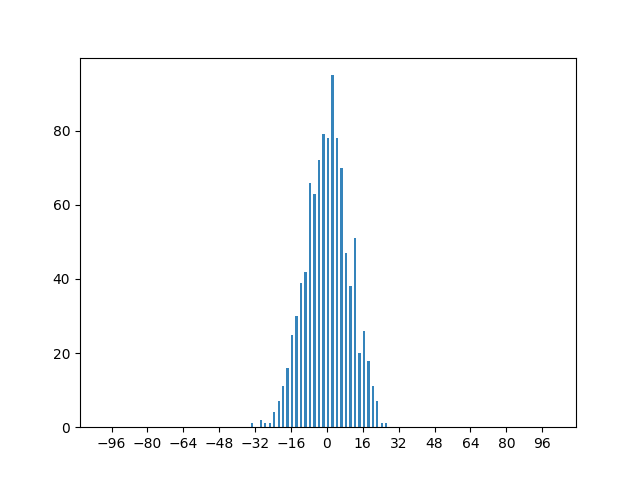
\includegraphics[width=0.6\textwidth]{../images/2d3.png}
    \caption{h=100}
\end{figure}
For h=100 alone, for better visibility, I have also written code with bins set to increment every 2 pockets. To observe the property of only even indexed bins being filled, simply replace range(-100, 102, 2) with range(-100, 102, 1).

\subsection{Task E}
\begin{align*}
    P_h[X=2i]=\frac{{{2k}\choose{i+k}}}{2^{2k}}
\end{align*}
Since the likelihood of a ball arriving at pocket i is equal to the likelihood of having i+k collisions which move it to the right within the 2k possible collisions overall.\\
Applying Stirling's approximations,
\begin{align*}
    P_h[X=2j] &\approx \frac{k^{2k}\sqrt{4\pi k}}{(k+j)^{k+j}\sqrt{2\pi (k+j)}(k-j)^{k-j}\sqrt{2\pi (k-j)}}\\
    &\approx \frac{k^{2k}\sqrt{2k}(k-j)^j}{(k^2-j^2)^{k}\sqrt{2\pi (k^2-j^2)}(k+j)^j}\\
    &\approx \frac{1}{\sqrt{\pi k}}\frac{k^{2k}(k-j)^{j}}{(k^2)^k(k+j)^{j}} && \text{(By approximating $k^2 - j^2 \approx j^2$)}\\
    &= \frac{1}{\sqrt{\pi k}}\left(1-\frac{2j}{k+j}\right)^j
\end{align*}

Now, we independently approximate $\left(1-\frac{2j}{k+j}\right)^j$ by taking its logarithm and using the property that for small x, $\ln(1-x) \approx -x$.
\begin{align*}
    \ln\left(\left(1-\frac{2j}{k+j}\right)^j\right) &= j\ln\left(1-\frac{2j}{k+j}\right)\\
    &\approx -\frac{2j^2}{k+j}\\
    \left(1-\frac{2j}{k+j}\right)^j&\approx e^{-\frac{2j^2}{k}}\\
\end{align*}
Setting $i=2j$ as required, we get 
\begin{align*}
    P_h[X=i]&\approx \frac{1}{\sqrt{\pi k}}e^{-\frac{i^2}{2k}}\\
    &= \frac{1}{\sqrt{\pi k}}e^{-\frac{i^2}{h}}
\end{align*}
As required.